\chapter{Results}

\section{Target archived}

The goals to archive include both logical and technical target. 
The improvements reached by thesis development are the following ones:

\newline
The main target to reach is to improve Value Chain \footnote{This process includes the following phases: design and 
development of the product,raw materials management, production, shipping, selling and final use} value of the 
overall system.
\newline
The goal could be split inside \textbf{Technical Goal} and \textbf{Logical Goal}.

\begin{outline}
    \1 \textbf{Technical Goal}
    \2 \textbf{CrossChain Interaction}: Integrates into the same application both permissioned and permissionless 
    Blockchain networks. The integration is done application side. Some API endpoints start transactions in both 
    networks, one over Fabric network and the other one over Ethereum.
    \2 \textbf{Traceability}: This goal is archived implementing smart contracts, Hyperledger Fabric side,
    that tracks all the clothes box and store the entire transactions passed over the system. 
    
    \1 \textbf{Logical Goal}
    \2 \textbf{Supply Chain}: The target is to simplify the supply chain process, all the steps inside the chain
    are handled as transactions, stored over the ledger and updating world state and smart contract data. 
    \2 \textbf{Sustainability}: The entire process aims to support sustainability. Thanks to traceability feature,
    it is possible to follow the lifetime of the clothes until they finish to Producer, that performs the 
    material recycling in order to produce new upcycled clothes.   
    \2 \textbf{Counterfeiting}: Assign a UID to each clothes produced it is possible to fight the Counterfeiting 
    implementing new features such as the clothes registrations. In that way it is possible to have a secure register 
    containing all the clothes.
\end{outline}

\section{Use Case Test}

\subsection{Use Case 1 - Unit Test 1}

\subsubsection{Send Box and Evaluation}

Performing the Test over the Use Case 1 about the send box and evaluation processes. The following
figures show the results over the call of the related methods and how the application works. 

\textbf{Figure \ref{fig:user-send-box}} shows the log when User performs the \textit{Send Box} action.

\begin{figure}[h!]
	\centering
    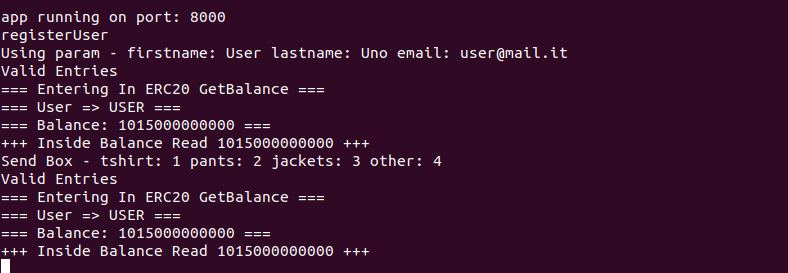
\includegraphics[totalheight=4cm]{img/test/test1/user-send-box.png}
	\caption{User Send Box}
	\label{fig:user-send-box}
\end{figure}

Once the Box Request was successfully sent, the smart contract is invoked and the transaction is 
performed. Admin could visualize the pending box requests to be evaluated. Then the Reclothes Admin, UI side,
insert the value amount of the tokens and start the evaluation process.
\newline
\textbf{Figures \ref{fig:init-tx-reclothes-user}} and \textbf{\ref{fig:tx-reclothes-user}} 
shows the Fabric Transaction performed then the initialization of the Ethereum transaction. In the end, once 
the eth transaction was performed, the etherscan link associated with the related TransactionHash, allow the 
user to see the transaction history and info.

\begin{figure}[h!]
	\centering
    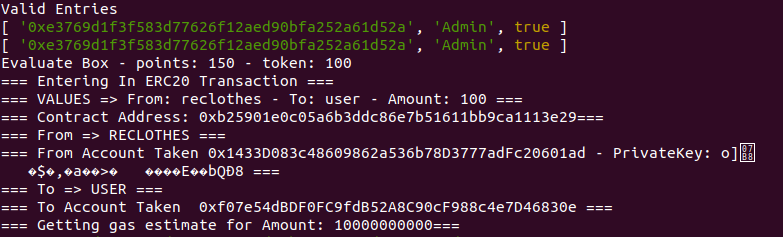
\includegraphics[totalheight=4cm]{img/test/test1/init-tx-RU.png}
	\caption{Init Transaction from Reclothes to User}
	\label{fig:init-tx-reclothes-user}
\end{figure}

\begin{figure}[h!]
	\centering
    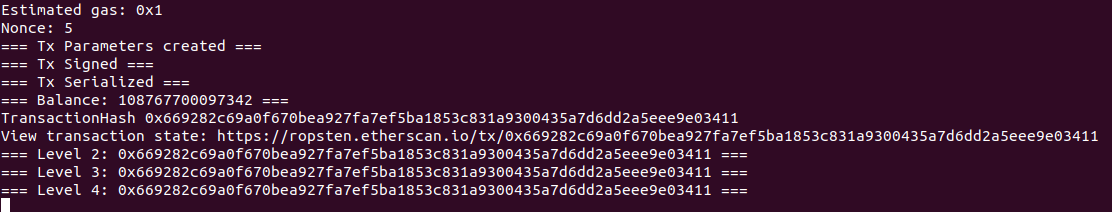
\includegraphics[totalheight=3cm]{img/test/test1/performed-tx-RU.png}
	\caption{Init Transaction from Reclothes to User}
	\label{fig:tx-reclothes-user}
\end{figure}

Figure \ref{fig:fabric-tx} and Figure \ref{fig:eth-tx} shows the proof of the transactions succeed. 
The first Figure shows the User page that allows visualizing the history of transactions done and all related 
requests. The second one shows the etherscan page with all the information about Ethereum's transaction, in 
this case from Reclothes eth Account to User Account.

\begin{figure}[h!]
	\centering
    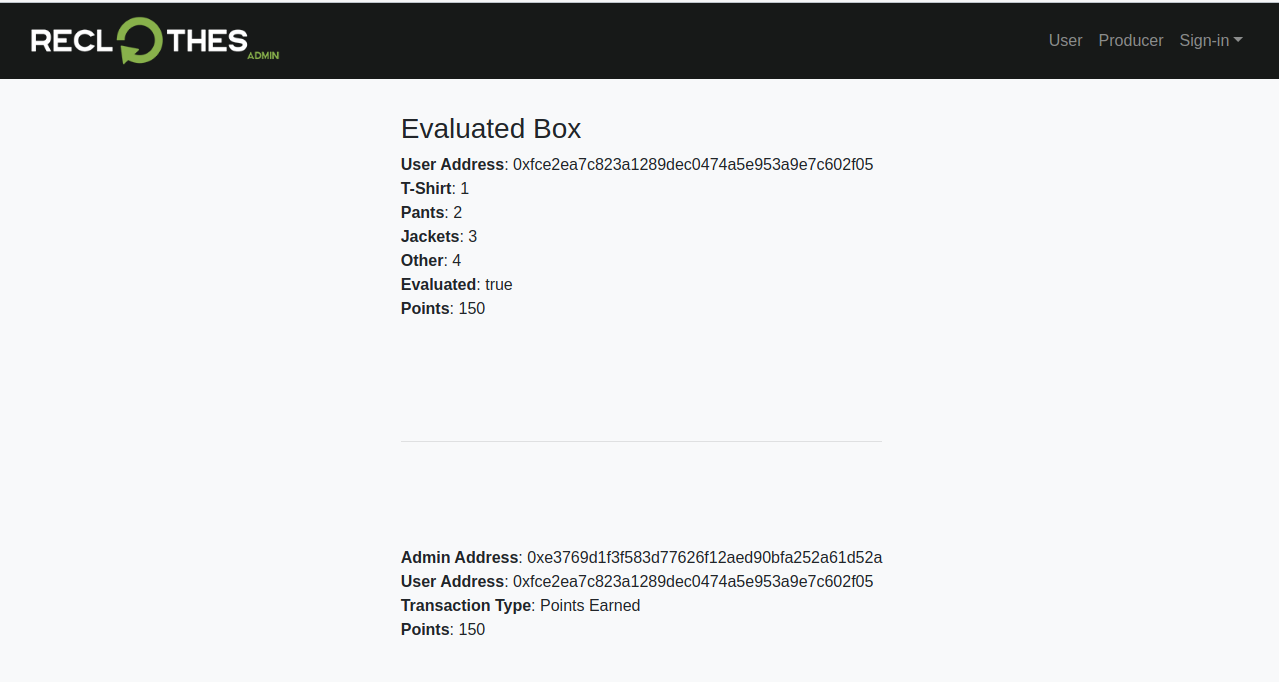
\includegraphics[totalheight=7cm]{img/test/test1/fabrix-tx.png}
	\caption{Fabric transaction history}
	\label{fig:fabric-tx}
\end{figure}

\begin{figure}[h!]
	\centering
    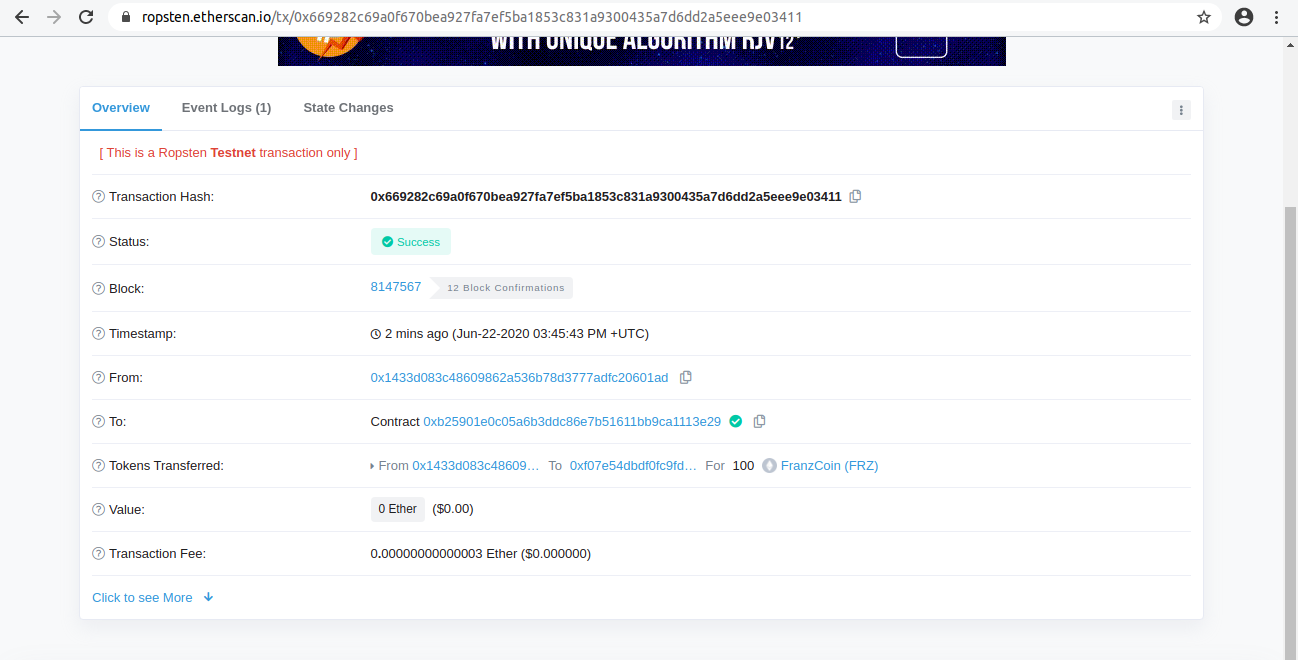
\includegraphics[totalheight=7cm]{img/test/test1/etherscan.png}
	\caption{Ethereum transaction over etherscan}
	\label{fig:eth-tx}
\end{figure}

\subsection{Use Case 1 - Unit Test 2}

\subsubsection{Purchase Item}

The \textbf{Figures \ref{fig:tx-user-reclothes}} shows the Purchase process. As the figure shows
there is, first of all, the Fabric transaction and then the Eth transaction. Once all
the previous checks are performed, the transaction from User account to Reclothes account starts. Once the 
transaction is performed the method prints the etherscan link to monitor the transaction and
all the related info. 

\begin{figure}[h!]
	\centering
    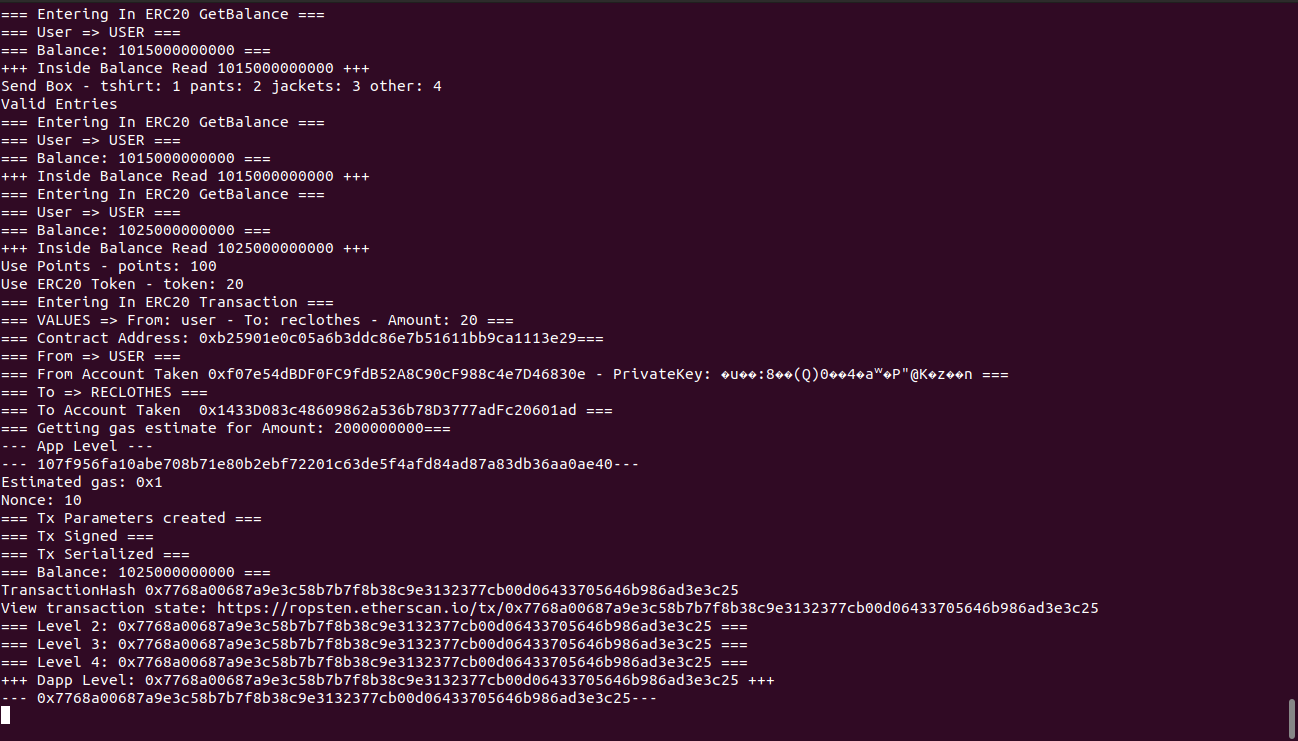
\includegraphics[totalheight=7cm]{img/test/test2/tx-user-reclothes.png}
	\caption{Transaction from User to Reclothes}
	\label{fig:tx-user-reclothes}
\end{figure}


\subsection{Use Case 2 - Unit Test 1}

To test the Use Case 2 I decided to track the behaviors of two processes:

\begin{outline}
    \1 \textbf{Send Old Material and Evaluation}: The Admin for Producer sends a box with inside the old materials
    to be recycled. Once the box arrived at Producer, then it is going to be evaluated and starts a 
    Regeneration Credits transaction from Producer to AdminP.

    \1 \textbf{Purchase Upcycled Material}: The Admin for Producer spends the earned Regeneration Credits
    to purchase by Producer recycled materials. The purchase options right now are three:
    \2 \textbf{Small Box}: 50 Regeneration Credits for 5 upcycled items.
    \2 \textbf{Medium Box}: 150 Regeneration Credits for 15 upcycled items.
    \2 \textbf{Big Box}: 200 Regeneration Credits for 40 upcycled items.
\end{outline}

\subsubsection{Send Old Material and Evaluation}

The \textbf{Figures \ref{fig:send-old-clothes}} shows the log of the send old clothes process.
In that case is sent a box with inside: 
\begin{outline}
    \1 \textbf{t-shirt}: 10
    \1 \textbf{pants}: 20
    \1 \textbf{jacket}: 10
    \1 \textbf{other}: 10
\end{outline}

\begin{figure}[h!]
	\centering
    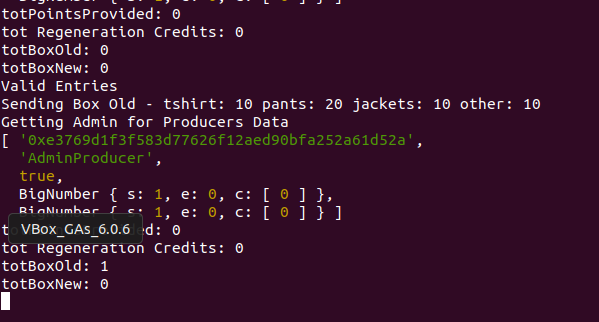
\includegraphics[totalheight=6cm]{img/test/usecase2/0-send-old-clothes.png}
	\caption{Admin Send old clothes}
	\label{fig:send-old-clothes}
\end{figure}

Once the box is sent, the evaluation process starts. The Producer evaluates materials received
and issue Regeneration Credits amount that Admins could spend when need, to purchase
recycled items. The \textbf{Figure \ref{fig:1-box-tobe-evaluate.png}} shows the page used
to perform evaluation Process by Producer. In that case I set a Regeneration Credits amount
of 1200. The \textbf{Figure \ref{fig:evaluation-old-clothes}} shows the output of the evaluation process.
\\
Once the evaluation process is archived and the Regeneration Credits is sent
from Producer to Admin. The \textbf{Figure \ref{fig:evaluation-old-clothes}} shows the info update
of the Admin for Producer.

\begin{figure}[h!]
	\centering
    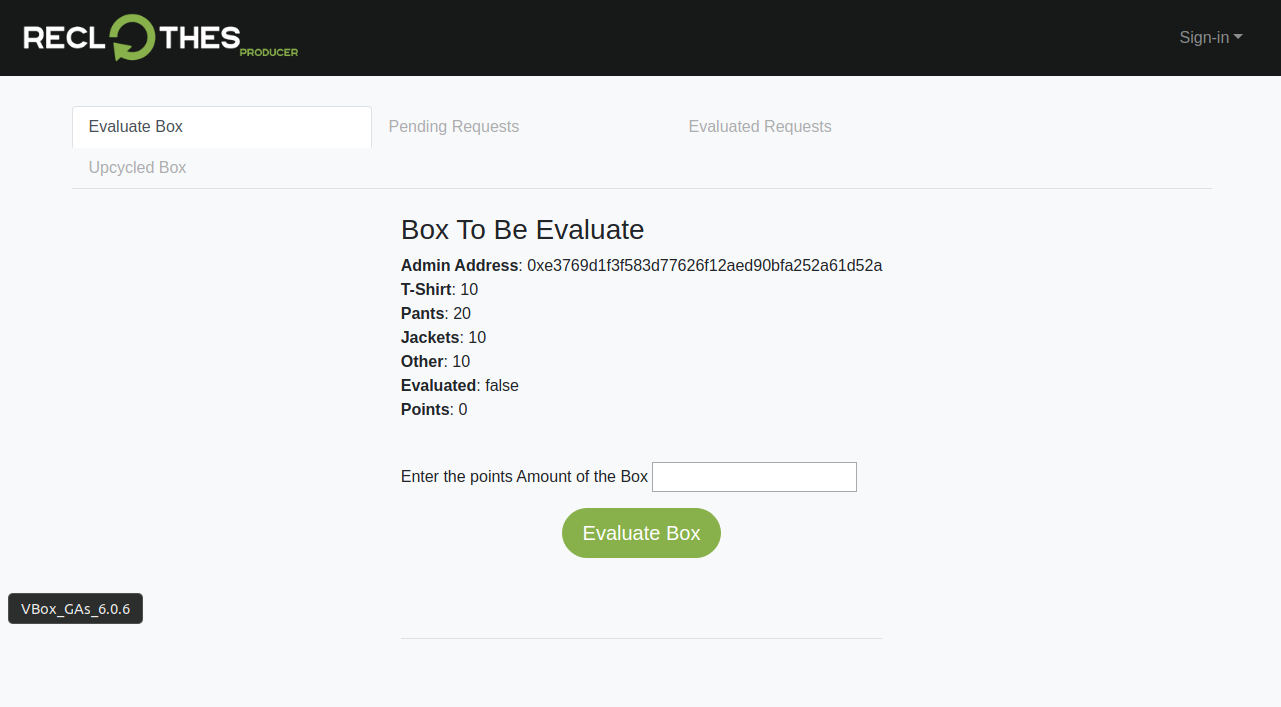
\includegraphics[totalheight=7cm]{img/test/usecase2/1-box-tobe-evaluate.png}
	\caption{Box to be evaluated}
	\label{fig:box-tobe-evaluate}
\end{figure}

\begin{figure}[h!]
	\centering
    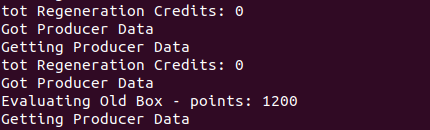
\includegraphics[totalheight=4cm]{img/test/usecase2/2-evaluation.png}
	\caption{Producer Evaluate old materials}
	\label{fig:evaluation-old-clothes}
\end{figure}

\begin{figure}[h!]
	\centering
    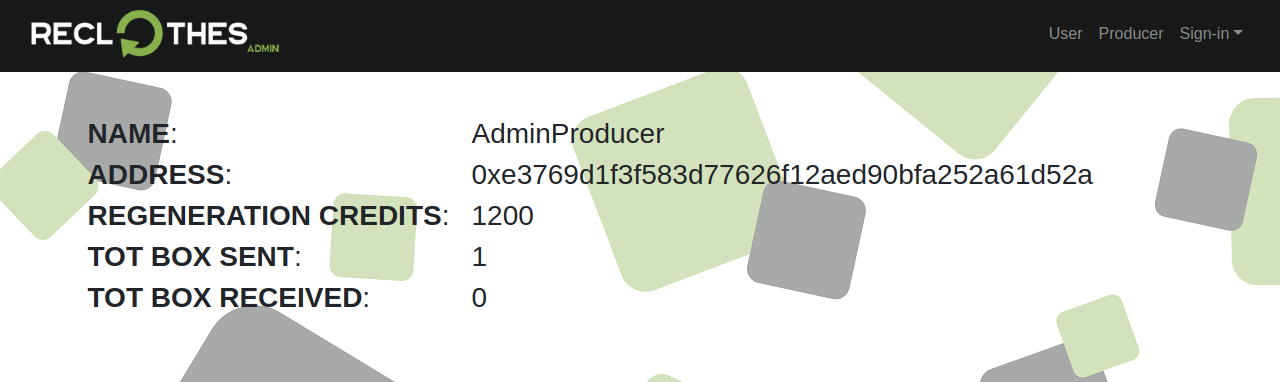
\includegraphics[totalheight=4cm]{img/test/usecase2/3-credits-received.png}
	\caption{Admin Info update}
	\label{fig:credits-received}
\end{figure}

\subsubsection{Purchase Upcycled Material}
 
Once the Admin sent the box with old clothes and the evaluation process is archived, Admin has a 
Regeneration Credits amount to spend purchasing upcycled clothes by Producer and then resell them
inside the platform store. In our test case, we purchase a \textbf{Middle Box} spending an amount 
of 150 Regeneration Credits.
\\
The \textbf{Figure \ref{fig:buy-recycled-clothes}} shows the output of the purchase process and the 
Tot Regeneration Credits update once the purchase box process is performed.
\\
The \textbf{Figure \ref{fig:producer-infos}} shows the update of Producer Information,
the circulating Regeneration Credits amount is changed and the Tot Box New number is updated.

\begin{figure}[h!]
	\centering
    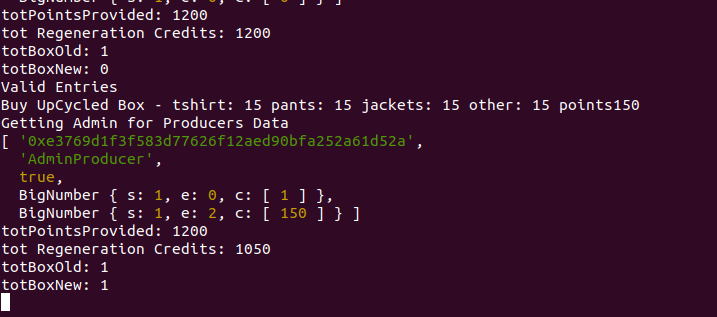
\includegraphics[totalheight=5cm]{img/test/usecase2/4-buy-recycled-clothes.png}
	\caption{Purchase Recycled Clothes}
	\label{fig:buy-recycled-clothes}
\end{figure}

\begin{figure}[h!]
	\centering
    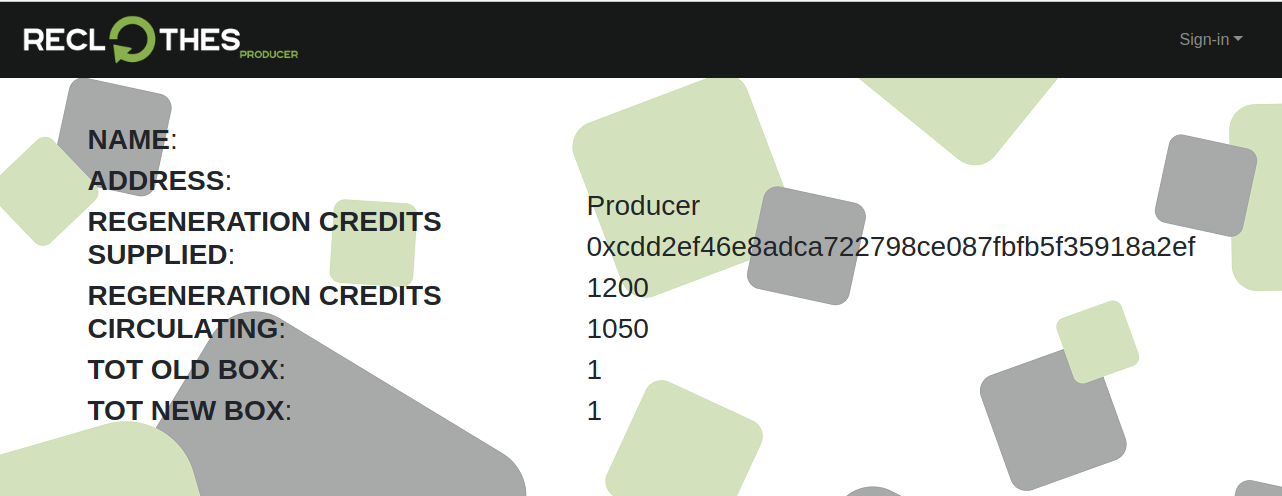
\includegraphics[totalheight=5cm]{img/test/usecase2/5-producer-info-update.png}
	\caption{Producer Infos Update}
	\label{fig:producer-infos}
\end{figure}